\subsection{\label{sec:level2}One x-point}
In the case of the primary x-point, we define N to be in the direction of decreasing psi towards the magnetic-axis, and S to be in the direction of decreasing psi towards the private-flux region. We assign a Point object for the N and S $(r,z)$ coordinates some small $\epsilon$ distance away from the primary x-point in order to provide the LineTracing class a starting point towards the magnetic-axis and private-flux region. To define E, W, NE, NW, SE, and SE, we simply apply the appropriate rotations to the established N and S directions of the primary x-point. The above results in a group of Point objects located a distance $\epsilon$ away from the primary x-point.\\ \indent
To highlight the significance of this convention, consider an SNL divertor configuration. Using the primary x-point N-S-E-W defintions used above, it can be seen that the to trace the primary separatrix, we simply perform LineTracing from the SW, SE, NW, and NE directions. This holds for both LSN and USN cases. Going further, we no longer rely on a notion of ``inner" and ``outer" for target plates, and can now utilize a general N-S-E-W direction to specify which target plate we are speaking of. In a typical LSN case, the ``inner" target plate is equivalently ``SW" of the primary x-point. Similarly, the ``outer" target plate is equivalently ``SE" of the primary x-point. We refer to these plates in the INGRID parameter file and documentation as ``plate\_W1" and ``plate\_E1". The W and E correspond to the ``SW" and ``SE" directions, whereas the ``1" indicates these plates correspond to the primary x-point dubbed ``xpt1".
\begin{figure}[H]
    \centering
    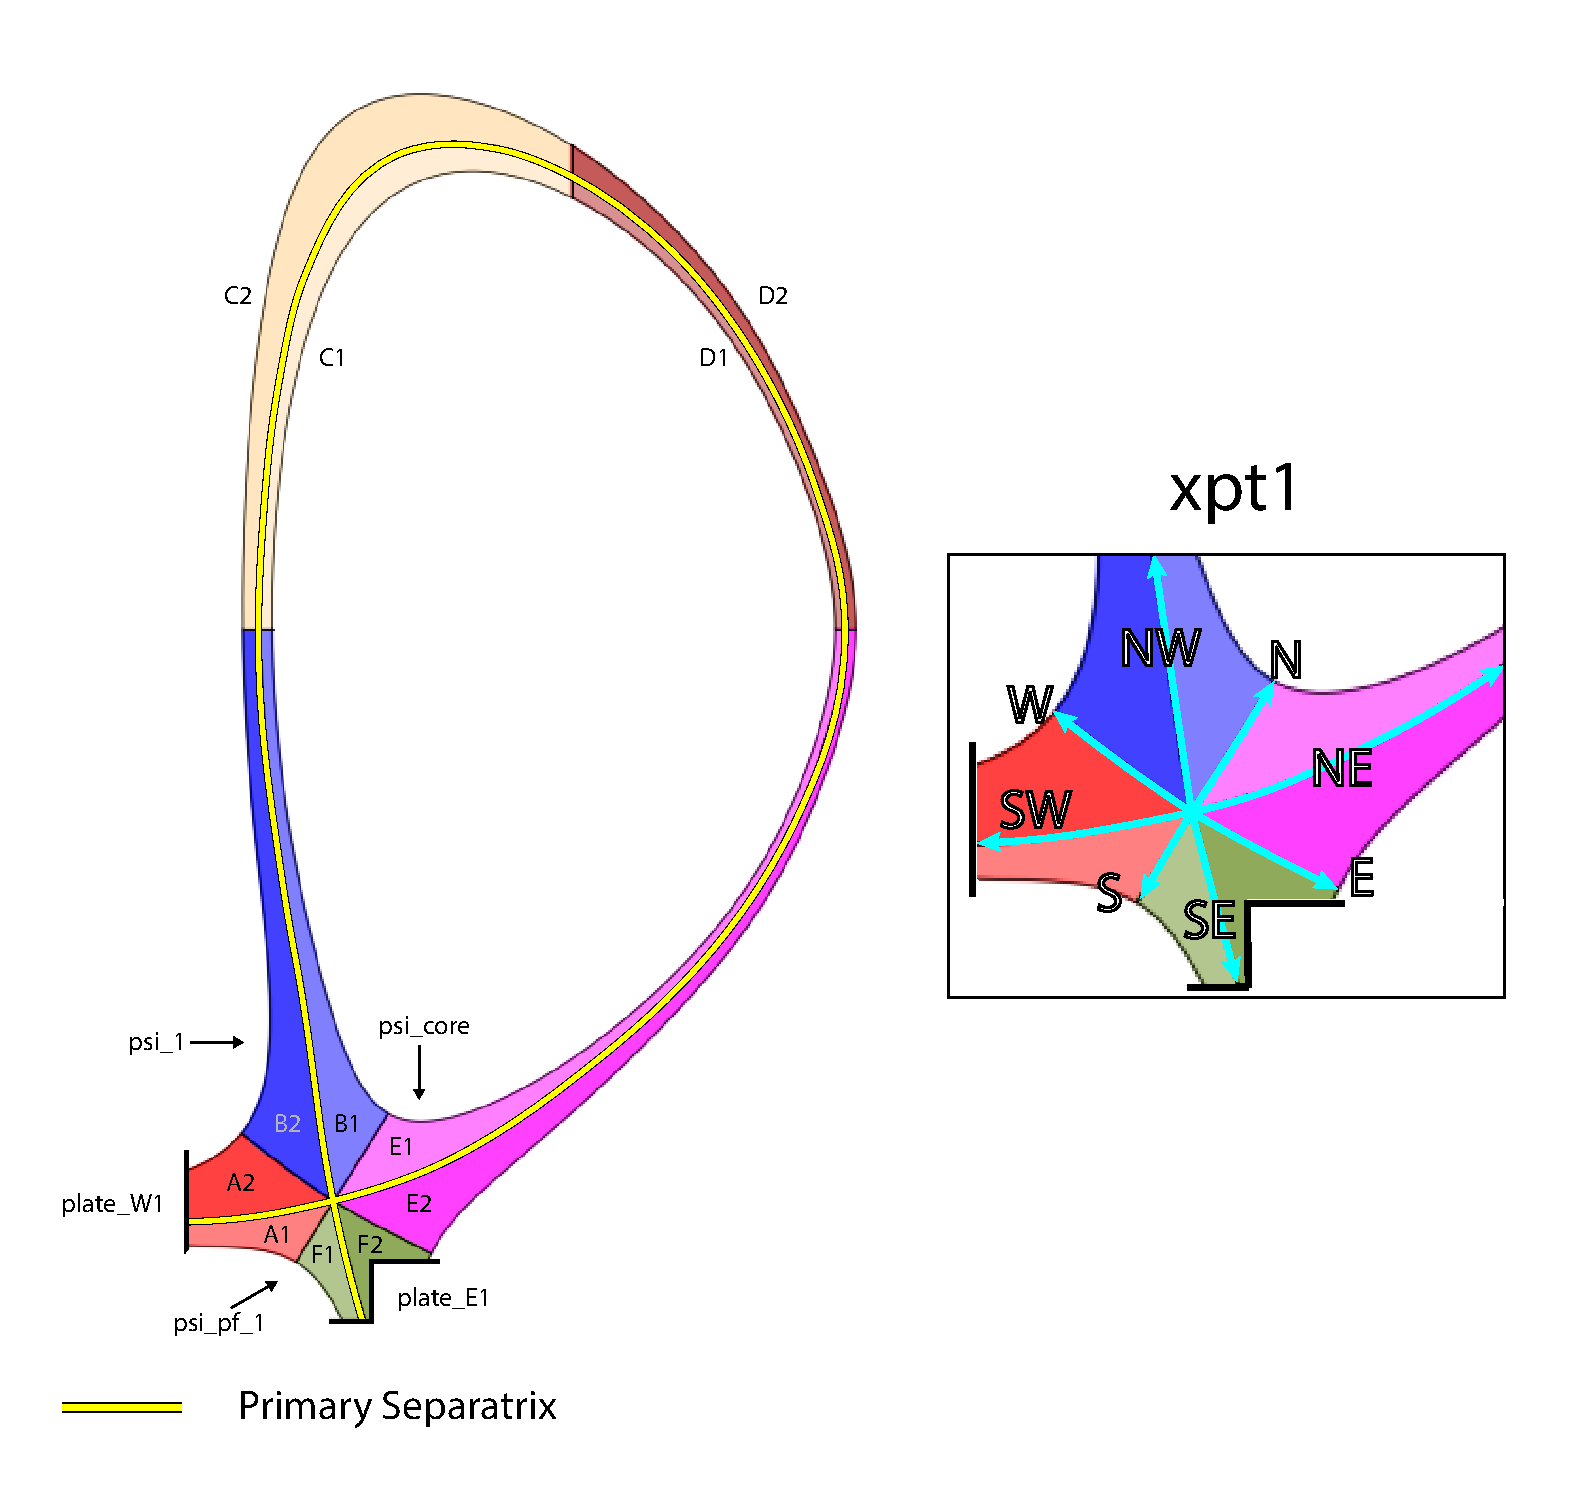
\includegraphics[width=\linewidth]{figures/xpt_1_directions.pdf}
    \caption{An SNL divertor configuration illustrating the primary x-point's N-S-E-W labeling convention.}
    \label{fig:xpt_1_directions}
\end{figure}